% Ilustrasi demo SeBatt: susunan meja dan tiga adegan.
% Kompilasi: tectonic -X compile alur-demo.tex  (atau latexmk -pdf alur-demo.tex)
% PNG: pdftoppm -png -r 300 -singlefile alur-demo.pdf alur-demo
\documentclass[border=8pt]{standalone}
\usepackage[T1]{fontenc}
\usepackage[scaled=0.92]{helvet}
\renewcommand{\familydefault}{\sfdefault}
\usepackage{tikz}
\usetikzlibrary{positioning,arrows.meta,calc,shapes.geometric}

\definecolor{ok}{HTML}{16A34A}
\definecolor{bad}{HTML}{DC2626}
\definecolor{ink}{HTML}{1F2937}

\tikzset{
  >={Stealth[length=2.2mm]},
  lbl/.style={font=\footnotesize, fill=white, inner sep=1.5pt},
  role/.style={font=\footnotesize\itshape, text=black!60},
  % Laptop: #1 = warna layar
  pics/laptop/.style={code={
    \fill[#1!10, draw=ink, line width=0.6pt, rounded corners=1pt] (-1.5,0.15) rectangle (1.5,2.1);
    \draw[ink, line width=0.6pt, fill=black!15] (-1.8,0) -- (1.8,0) -- (1.6,0.15) -- (-1.6,0.15) -- cycle;
  }},
  % Orang sederhana
  pics/person/.style={code={
    \draw[ink, line width=0.7pt] (0,0.75) circle (0.17);
    \draw[ink, line width=0.7pt] (0,0.58) -- (0,0.15) (0,0.15) -- (-0.15,-0.2) (0,0.15) -- (0.15,-0.2)
                                 (-0.22,0.42) -- (0.22,0.42);
  }},
}

\begin{document}
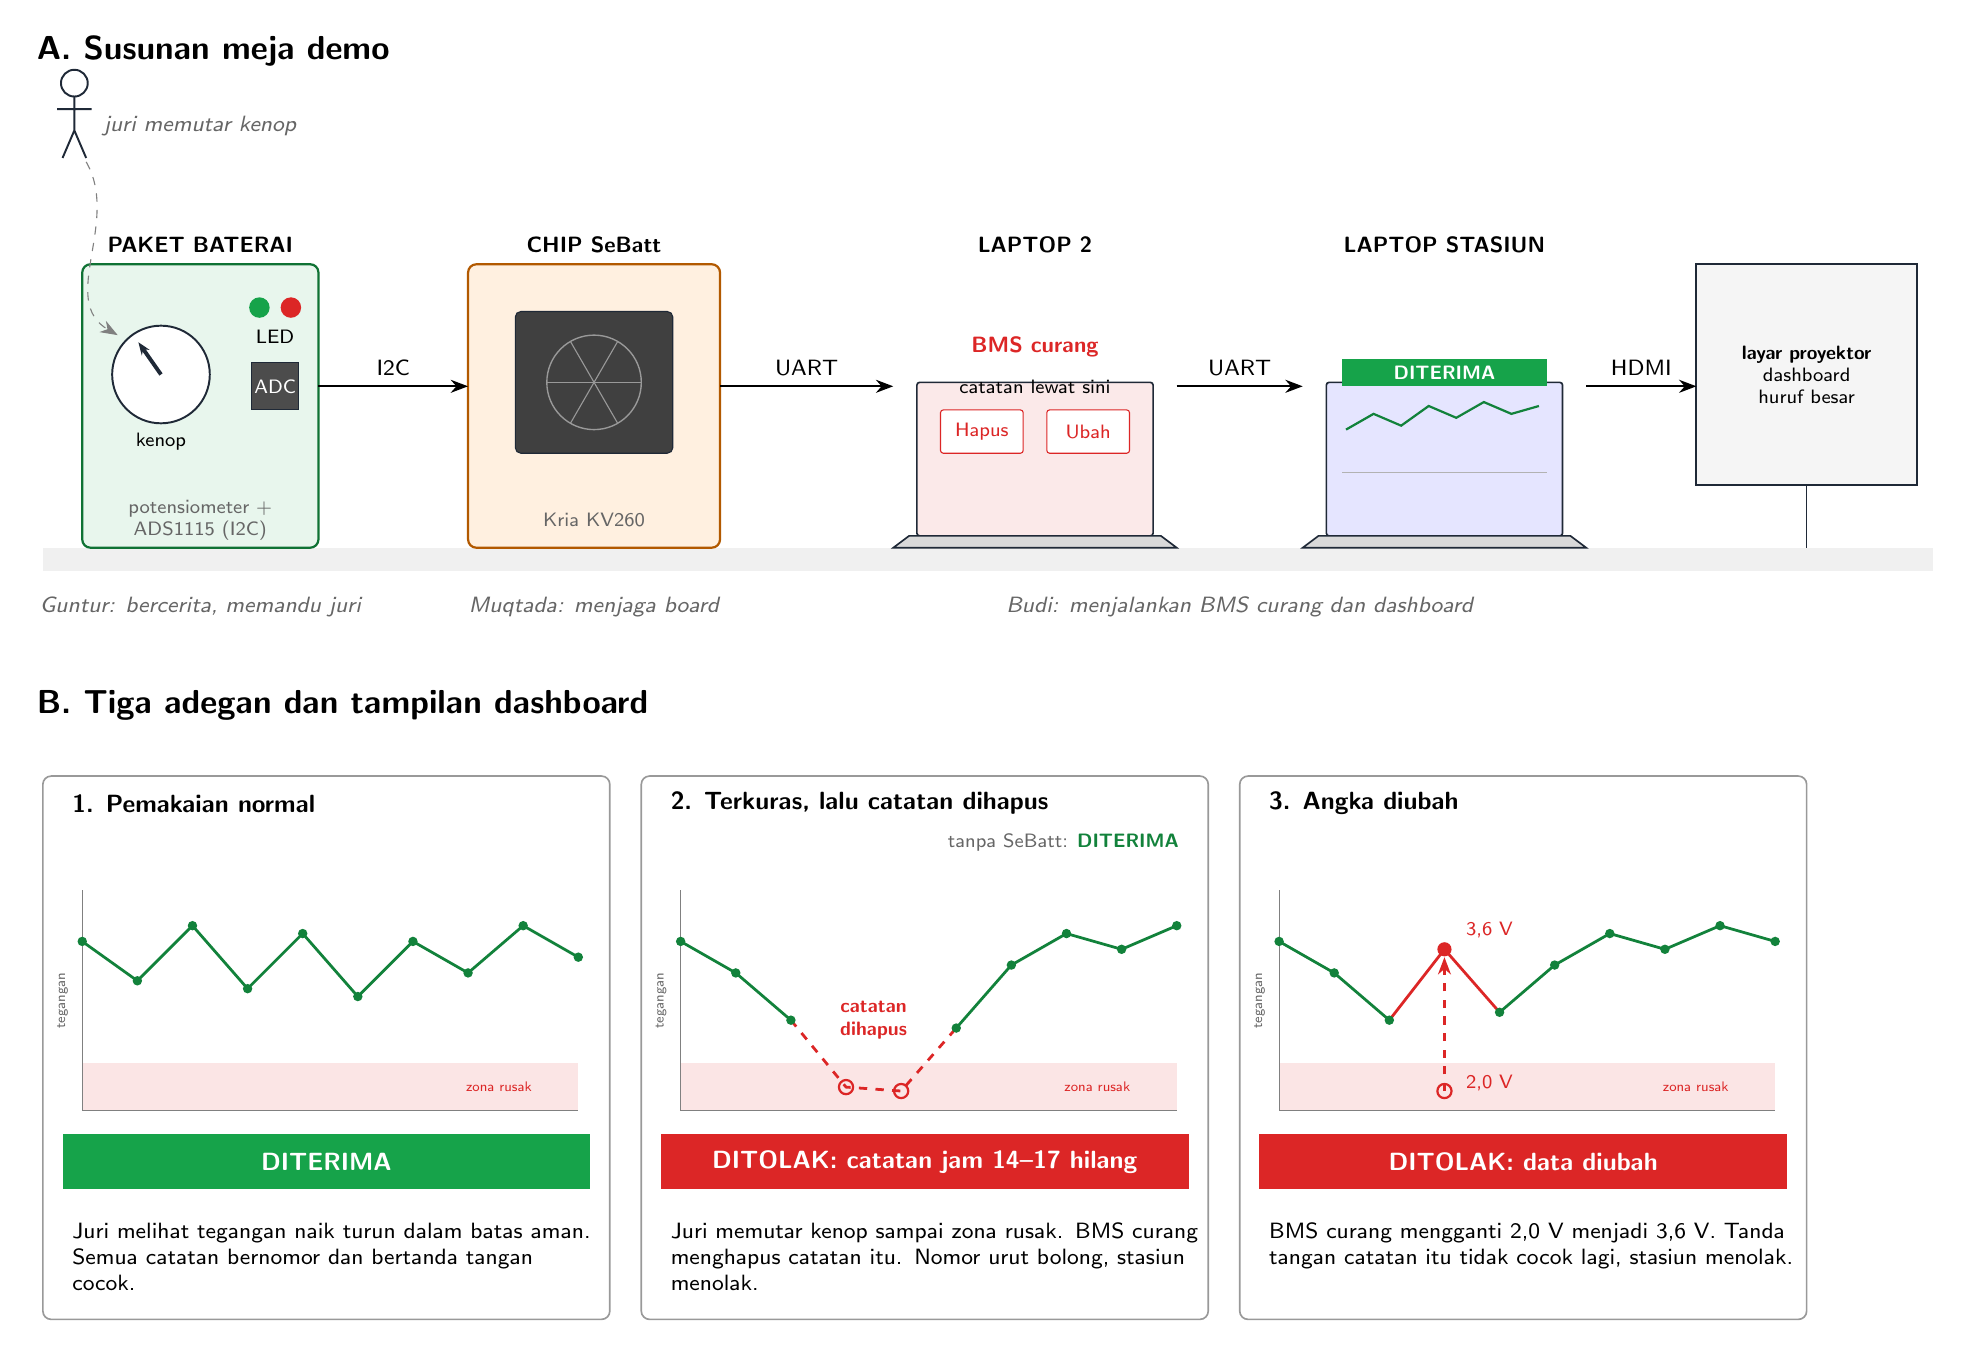
\begin{tikzpicture}[font=\small]

% =====================================================================
% A. Susunan meja
% =====================================================================
\node[font=\bfseries\large, anchor=west] at (-1.6,5.7) {A. Susunan meja demo};

% Meja
\fill[black!6] (-1.4,-0.9) rectangle (22.6,-0.6);

% --- Paket baterai
\node[font=\bfseries\footnotesize] at (0.6,3.25) {PAKET BATERAI};
\draw[ok!70!black, fill=ok!10, rounded corners=3pt, line width=0.8pt] (-0.9,-0.6) rectangle (2.1,3.0);
\draw[ink, fill=white, line width=0.7pt] (0.1,1.6) circle (0.62);
\draw[ink, line width=1.4pt, -{Stealth[length=1.6mm]}] (0.1,1.6) -- ++(125:0.5);
\node[font=\scriptsize] at (0.1,0.75) {kenop};
\draw[ink, fill=black!70] (1.25,1.15) rectangle (1.85,1.75);
\node[font=\scriptsize, text=white] at (1.55,1.45) {ADC};
\fill[ok] (1.35,2.45) circle (0.13);
\fill[bad] (1.75,2.45) circle (0.13);
\node[font=\scriptsize] at (1.55,2.08) {LED};
\node[font=\scriptsize, text=black!60, align=center] at (0.6,-0.25) {potensiometer +\\ADS1115 (I2C)};

% Juri memutar kenop
\pic at (-1.0,4.55) {person};
\node[role, anchor=west] at (-0.75,4.75) {juri memutar kenop};
\draw[->, black!50, dashed] (-0.85,4.3) to[out=-60,in=150] (-0.45,2.1);

% --- KV260
\node[font=\bfseries\footnotesize, align=center] at (5.6,3.25) {CHIP SeBatt};
\draw[orange!70!black, fill=orange!12, rounded corners=3pt, line width=0.8pt] (4.0,-0.6) rectangle (7.2,3.0);
\draw[ink, fill=black!75, rounded corners=2pt] (4.6,0.6) rectangle (6.6,2.4);
\draw[black!40, line width=0.5pt] (5.6,1.5) circle (0.6);
\foreach \a in {0,60,...,300} \draw[black!40] (5.6,1.5) -- ++(\a:0.6);
\node[font=\scriptsize, text=black!60] at (5.6,-0.25) {Kria KV260};

% --- Laptop BMS curang
\pic at (11.2,-0.6) {laptop=bad};
\node[font=\bfseries\footnotesize, text=bad] at (11.2,1.95) {BMS curang};
\draw[bad, fill=white, rounded corners=1pt] (10.0,0.6) rectangle (11.05,1.15);
\node[font=\scriptsize, text=bad] at (10.525,0.875) {Hapus};
\draw[bad, fill=white, rounded corners=1pt] (11.35,0.6) rectangle (12.4,1.15);
\node[font=\scriptsize, text=bad] at (11.875,0.875) {Ubah};
\node[font=\scriptsize] at (11.2,1.45) {catatan lewat sini};
\node[font=\bfseries\footnotesize] at (11.2,3.25) {LAPTOP 2};

% --- Laptop stasiun
\pic at (16.4,-0.6) {laptop=blue};
\node[font=\bfseries\footnotesize] at (16.4,3.25) {LAPTOP STASIUN};
\draw[black!30] (15.1,0.35) -- (17.7,0.35);
\draw[ok!80!black, line width=0.8pt] (15.15,0.9) -- (15.5,1.1) -- (15.85,0.95) -- (16.2,1.2) -- (16.55,1.05) -- (16.9,1.25) -- (17.25,1.1) -- (17.6,1.2);
\fill[ok] (15.1,1.45) rectangle (17.7,1.8);
\node[font=\scriptsize\bfseries, text=white] at (16.4,1.625) {DITERIMA};

% --- Proyektor
\draw[ink, fill=black!4, line width=0.7pt] (19.6,0.2) rectangle (22.4,3.0);
\draw[ink, line width=0.6pt] (21.0,0.2) -- (21.0,-0.6);
\node[font=\scriptsize\bfseries, align=center] at (21.0,1.6) {layar proyektor\\{\normalfont dashboard}\\{\normalfont huruf besar}};

% --- Kabel
\draw[->, line width=0.8pt] (2.1,1.45) -- node[lbl, above=2pt]{I2C} (4.0,1.45);
\draw[->, line width=0.8pt] (7.2,1.45) -- node[lbl, above=2pt]{UART} (9.4,1.45);
\draw[->, line width=0.8pt] (13.0,1.45) -- node[lbl, above=2pt]{UART} (14.6,1.45);
\draw[->, line width=0.8pt] (18.2,1.45) -- node[lbl, above=2pt]{HDMI} (19.6,1.45);

% --- Peran
\node[role] at (0.6,-1.35) {Guntur: bercerita, memandu juri};
\node[role] at (5.6,-1.35) {Muqtada: menjaga board};
\node[role] at (13.8,-1.35) {Budi: menjalankan BMS curang dan dashboard};

% =====================================================================
% B. Tiga adegan
% =====================================================================
\node[font=\bfseries\large, anchor=west] at (-1.6,-2.6) {B. Tiga adegan dan tampilan dashboard};

\newcommand{\panel}[3]{% #1 = x kiri, #2 = judul, #3 = keterangan
  \draw[black!40, fill=white, rounded corners=3pt, line width=0.6pt] (#1,-10.4) rectangle ++(7.2,6.9);
  \node[font=\bfseries\small, anchor=west] at ($(#1,-3.85)+(0.25,0)$) {#2};
  \node[font=\footnotesize, anchor=north west, text width=6.7cm, align=left, execute at begin node={\hyphenpenalty=10000\exhyphenpenalty=10000}] at ($(#1,-9.05)+(0.25,0)$) {#3};
  % sumbu grafik
  \fill[bad!12] ($(#1,-7.75)+(0.5,0)$) rectangle ($(#1,-7.15)+(6.8,0)$);
  \node[font=\tiny, text=bad, anchor=west] at ($(#1,-7.45)+(5.25,0)$) {zona rusak};
  \draw[black!50] ($(#1,-7.75)+(0.5,0)$) -- ($(#1,-7.75)+(6.8,0)$);
  \draw[black!50] ($(#1,-7.75)+(0.5,0)$) -- ($(#1,-4.95)+(0.5,0)$);
  \node[font=\tiny, rotate=90, text=black!60] at ($(#1,-6.35)+(0.25,0)$) {tegangan};
}

% --- Panel 1: normal
\panel{-1.4}{1. Pemakaian normal}{Juri melihat tegangan naik turun dalam batas aman. Semua catatan bernomor dan bertanda tangan cocok.}
\draw[ok!80!black, line width=1pt] (-0.9,-5.6) -- (-0.2,-6.1) -- (0.5,-5.4) -- (1.2,-6.2) -- (1.9,-5.5) -- (2.6,-6.3) -- (3.3,-5.6) -- (4.0,-6.0) -- (4.7,-5.4) -- (5.4,-5.8);
\foreach \x/\y in {-0.9/-5.6,-0.2/-6.1,0.5/-5.4,1.2/-6.2,1.9/-5.5,2.6/-6.3,3.3/-5.6,4.0/-6.0,4.7/-5.4,5.4/-5.8} \fill[ok!80!black] (\x,\y) circle (0.06);
\fill[ok] (-1.15,-8.75) rectangle (5.55,-8.05);
\node[font=\small\bfseries, text=white] at (2.2,-8.4) {DITERIMA};

% --- Panel 2: terkuras lalu dihapus
\panel{6.2}{2. Terkuras, lalu catatan dihapus}{Juri memutar kenop sampai zona rusak. BMS curang menghapus catatan itu. Nomor urut bolong, stasiun menolak.}
\draw[ok!80!black, line width=1pt] (6.7,-5.6) -- (7.4,-6.0) -- (8.1,-6.6);
\draw[bad, line width=1pt, dashed] (8.1,-6.6) -- (8.8,-7.45) -- (9.5,-7.5) -- (10.2,-6.7);
\draw[ok!80!black, line width=1pt] (10.2,-6.7) -- (10.9,-5.9) -- (11.6,-5.5) -- (12.3,-5.7) -- (13.0,-5.4);
\foreach \x/\y in {6.7/-5.6,7.4/-6.0,8.1/-6.6,10.2/-6.7,10.9/-5.9,11.6/-5.5,12.3/-5.7,13.0/-5.4} \fill[ok!80!black] (\x,\y) circle (0.06);
\foreach \x/\y in {8.8/-7.45,9.5/-7.5} \draw[bad, line width=0.8pt] (\x,\y) circle (0.09);
\node[font=\scriptsize\bfseries, text=bad, align=center] at (9.15,-6.6) {catatan\\dihapus};
\fill[bad] (6.45,-8.75) rectangle (13.15,-8.05);
\node[font=\small\bfseries, text=white] at (9.8,-8.4) {DITOLAK: catatan jam 14--17 hilang};
\node[font=\scriptsize, text=black!60, anchor=east] at (13.15,-4.35) {tanpa SeBatt: \textcolor{ok!80!black}{\textbf{DITERIMA}}};

% --- Panel 3: angka diubah
\panel{13.8}{3. Angka diubah}{BMS curang mengganti 2,0 V menjadi 3,6 V. Tanda tangan catatan itu tidak cocok lagi, stasiun menolak.}
\draw[ok!80!black, line width=1pt] (14.3,-5.6) -- (15.0,-6.0) -- (15.7,-6.6);
\draw[bad, line width=1pt] (15.7,-6.6) -- (16.4,-5.7) -- (17.1,-6.5);
\draw[ok!80!black, line width=1pt] (17.1,-6.5) -- (17.8,-5.9) -- (18.5,-5.5) -- (19.2,-5.7) -- (19.9,-5.4) -- (20.6,-5.6);
\foreach \x/\y in {14.3/-5.6,15.0/-6.0,15.7/-6.6,17.1/-6.5,17.8/-5.9,18.5/-5.5,19.2/-5.7,19.9/-5.4,20.6/-5.6} \fill[ok!80!black] (\x,\y) circle (0.06);
\draw[bad, line width=0.8pt, dashed, ->] (16.4,-7.5) -- (16.4,-5.8);
\fill[bad] (16.4,-5.7) circle (0.09);
\draw[bad, line width=0.8pt] (16.4,-7.5) circle (0.09);
\node[font=\scriptsize, text=bad, anchor=west] at (16.55,-7.4) {2,0 V};
\node[font=\scriptsize, text=bad, anchor=west] at (16.55,-5.45) {3,6 V};
\fill[bad] (14.05,-8.75) rectangle (20.75,-8.05);
\node[font=\small\bfseries, text=white] at (17.4,-8.4) {DITOLAK: data diubah};

\end{tikzpicture}
\end{document}
